\documentclass[conference]{IEEEtran}
\IEEEoverridecommandlockouts
% The preceding line is only needed to identify funding in the first footnote. If that is unneeded, please comment it out.
\usepackage{cite}
\usepackage{amsmath,amssymb,amsfonts}
\usepackage{algorithmic}
\usepackage{graphicx}
\usepackage{textcomp}
\usepackage{xcolor}
\def\BibTeX{{\rm B\kern-.05em{\sc i\kern-.025em b}\kern-.08em
    T\kern-.1667em\lower.7ex\hbox{E}\kern-.125emX}}
\begin{document}

\title{Optimizing Knowledge Extraction and Knowledge Retrieval in RAG for Mental Health Chatbot}

\author{\IEEEauthorblockN{1\textsuperscript{st} Ega Rizky Setiawan}
    \IEEEauthorblockA{
        \textit{Department of Electrical and} \\
        \textit{Information Engineering} \\
        \textit{Faculty of Engineering} \\
        \textit{Universitas Gadjah Mada}\\
        Yogyakarta, Indonesia \\
        ega.rizky.setiawan@mail.ugm.ac.id}
    \and
    \IEEEauthorblockN{2\textsuperscript{nd} Bimo Sunarfri Hantono}
    \IEEEauthorblockA{
        \textit{Department of Electrical and} \\
        \textit{Information Engineering} \\
        \textit{Faculty of Engineering} \\
        \textit{Universitas Gadjah Mada}\\
        Yogyakarta, Indonesia \\
        bhe@ugm.ac.id}
    \and
    \IEEEauthorblockN{3\textsuperscript{rd}  Guntur Dharma Putra}
    \IEEEauthorblockA{
        \textit{Department of Electrical and} \\
        \textit{Information Engineering} \\
        \textit{Faculty of Engineering} \\
        \textit{Universitas Gadjah Mada}\\
        Yogyakarta, Indonesia \\
        gdputra@ugm.ac.id}
}

\maketitle

\begin{abstract}
    The use of chatbots as an accessible facilities for mental health support faces a crucial challenge regarding information accuracy.
    Common chatbot architectures, such as the conventional Retrieval-Augmented Generation (RAG) approach (Naive RAG) which relies on document chunks, carry a risk of generating misinformation and hallucinations due to a lack of comprehensive contextual understanding.
    This research aims to address this issue by designing, implementing, and evaluating a RAG architecture enriched with a structured knowledge base in the form of a Knowledge Graph (KG).
    The proposed methodology focuses on three main pillars that is the design of a RAG architecture that integrates a KG to ensure consistency and accuracy, the optimization of the Knowledge Extraction (KE) process using an LLM to build the KG from mental health literature, and the evaluation of various Knowledge Retrieval (KR) methods to find the most relevant information.
    Experimental results show that the RAG-KG architecture significantly outperforms the Naive RAG approach, demonstrated by an 8\% increase in correctness, a 4\% increase in faithfulness, and a 17\% increase in relevancy.
    This study confirms that the use of a Knowledge Graph, built and accessed through an optimized method, is a robust approach to enhance the reliability and security of chatbots.
    The result is a system capable of delivering more factual, relevant, and evidence-based mental health information, while minimizing the risk of hallucinations.
\end{abstract}

\begin{IEEEkeywords}
    RAG, knowledge graph, knowledge extraction, knowledge retrieval, chatbot, mental health, LLM
\end{IEEEkeywords}

\section{Introduction}
Mental health is a critical component of individual and societal well-being, yet access to quality care remains a significant challenge globally and in Indonesia \cite{INAMHS2022}.
Factors such as social stigma, a shortage of professionals, and high costs create a substantial gap between the need for and the availability of services \cite{WHO2022MentalHealth}.
Digital solutions, particularly AI-powered chatbots, offer a promising avenue to provide accessible, first-line psychological support \cite{CBTWoebotTest}.
However, standard Large Language Model (LLM) powered chatbots are prone to factual inaccuracies and "hallucinations"—generating plausible but incorrect information.
This risk is unacceptable in the sensitive domain of mental health. To mitigate this, the Retrieval-Augmented Generation (RAG) architecture has been proposed, which grounds LLM responses in external knowledge sources \cite{Lewis2021RAGKnowledgeIntensiveNLP}.
While conventional RAG systems using unstructured text chunks are an improvement, they often struggle to capture the complex, interconnected nature of knowledge in specialized domains like mental health.
A Knowledge Graph (KG), which represents information as a network of entities and their relationships, offers a more structured and powerful foundation for reasoning and precise information retrieval \cite{Edge2025LocalGlobalGraphRAG}.
This paper addresses the limitations of existing systems by proposing an optimized RAG architecture based on a Knowledge Graph. Our primary contributions are:
\begin{itemize}
    \item The design and implementation of a KG-RAG architecture that significantly enhances the factual accuracy and consistency of a mental health chatbot.
    \item An optimized Knowledge Extraction pipeline using an LLM with few-shot prompting to effectively construct a domain-specific KG from Indonesian mental health literature.
    \item A comprehensive evaluation of various Knowledge Retrieval strategies, demonstrating that adaptive graph traversal methods outperform standard vector search and baseline RAG.
\end{itemize}

\section{Related Work}

The development of conversational agents has evolved through several paradigms.
Early systems like ELIZA were rule-based, offering high predictability but suffering from rigidity and poor scalability \cite{Weizenbaum1966ELIZA}.
With the advent of LLMs, fine-tuning became a popular approach to adapt models to specific domains \cite{yu2024FineTuneOnMentalHealthChatbotExperimental}.
While effective at capturing style and specific knowledge, fine-tuning is computationally expensive, requires large, high-quality datasets, and struggles to incorporate new information without complete retraining, while still being susceptible to hallucination.

The RAG framework, introduced by Lewis et al., addresses the issue of static knowledge by combining a retriever with a generator \cite{Lewis2021RAGKnowledgeIntensiveNLP}.
The retriever fetches relevant text passages from a corpus, which are then used as context by an LLM to generate a factually grounded response.
This approach has proven effective in knowledge-intensive NLP tasks.

More recently, researchers have explored replacing unstructured text corpora with Knowledge Graphs as the knowledge source for RAG. A KG models entities (e.g., "Depression") and relationships (e.g., "is treated by") explicitly, enabling more precise retrieval and complex reasoning than is possible with simple document chunks \cite{Edge2025LocalGlobalGraphRAG}.
The GraphRAG approach, for instance, leverages graph structures and community detection to provide global context for summarization tasks.
Our work builds on this foundation by focusing specifically on optimizing the extraction and retrieval mechanisms for a question-answering chatbot in the mental health domain.

\section{System Model}
Our proposed system consists of two core pipelines: the Knowledge Graph Construction Pipeline, responsible for offline data processing, and the Retrieval and Generation Pipeline, responsible for online query handling.

\subsection{Knowledge Graph Construction Pipeline}
The KG is built from a corpus of Indonesian mental health documents, including technical guides from the Ministry of Health and articles from trusted sources.
The process, illustrated in Fig.~\ref{fig:knowledge-extraction-pipeline}, involves several automated steps.

\begin{figure}[htbp]
    \centerline{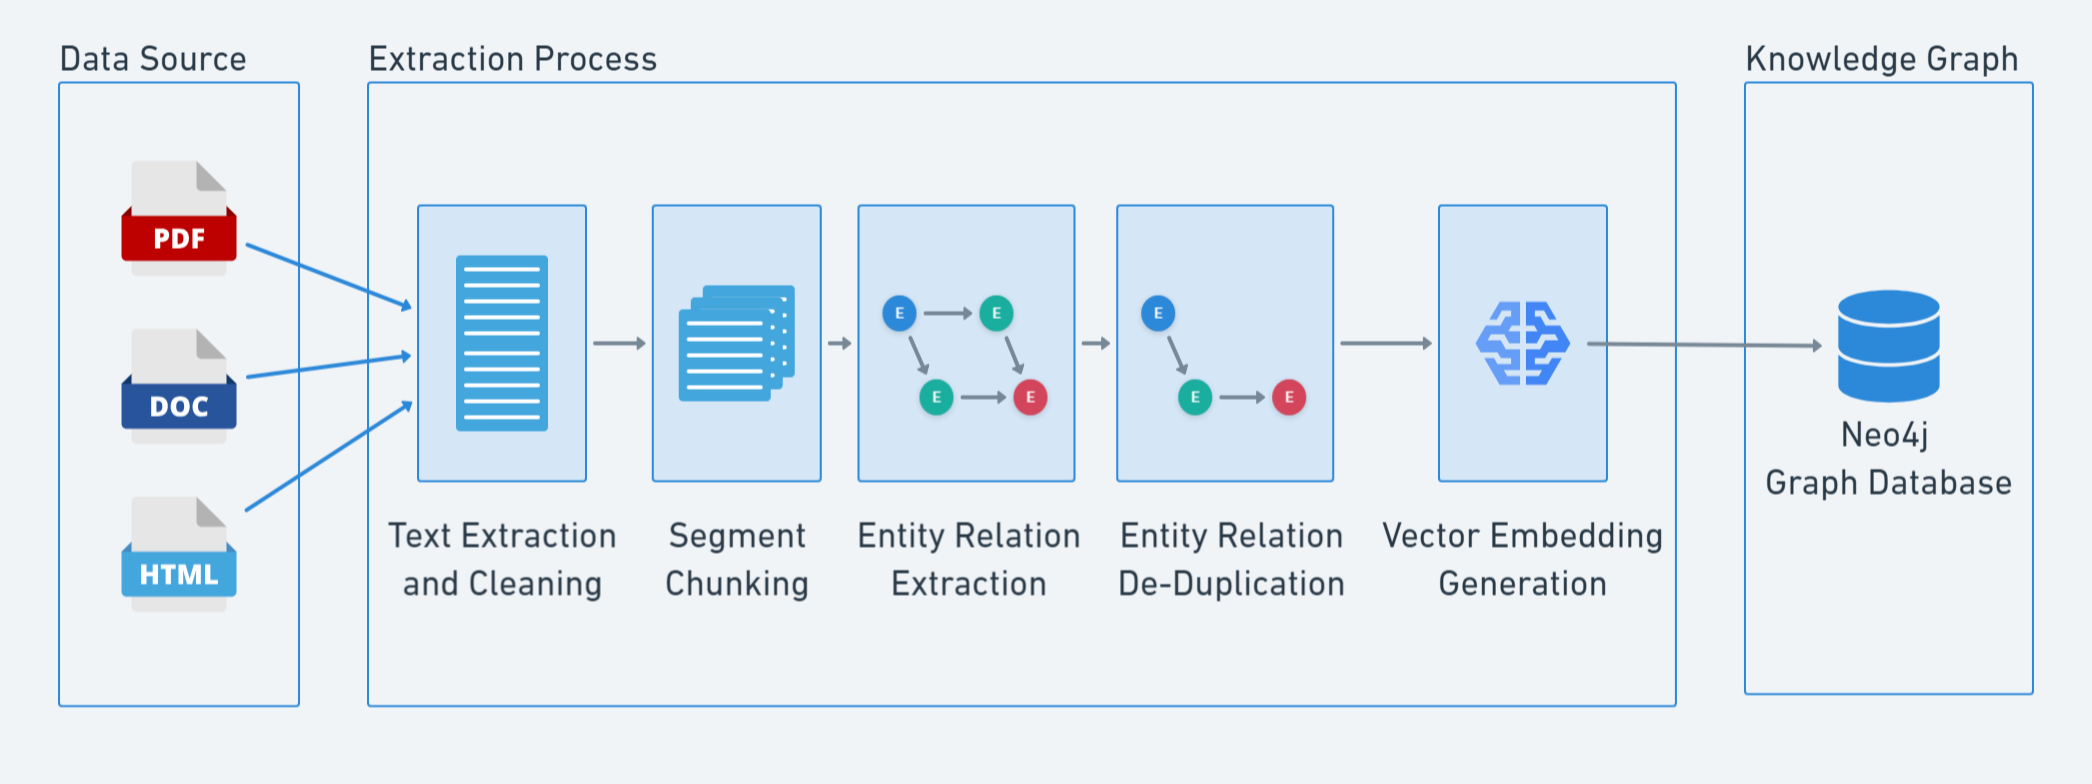
\includegraphics[width=0.45\textwidth]{knowledge-extraction-flow.png}}
    \caption{Knowledge Extraction pipeline.}
    \label{fig:knowledge-extraction-pipeline}
\end{figure}

\begin{itemize}
    \item Text Extraction \& Chunking: Text is extracted from source files (PDF, DOCX, HTML).
          To manage long documents and preserve context, we employ structural chunking, where documents are split based on semantic sections (e.g., chapters or headings) rather than fixed-size blocks.
          This approach aims to avoid incomplete context due to defect in document slicing.
          Incompleteness can lead to LLM failure in understanding a concept in document.

    \item Entity \& Relation Extraction: We use a powerful LLM (Google Gemini 2.5 Flash) to extract entities (e.g., Gangguan Mental, Terapi Psikologis) and their relationships from each text chunk.
          This is guided by a designed few-shot prompt that provides the LLM with instructions, a predefined ontology of entity and relation types, and examples of input and desired result to ensure high-quality, structured output in JSON format.

    \item Entity Resolution \& Embedding: Extracted entities are deduplicated and merged to maintain consistency across the KG.
          The descriptions of duplicate entities are combined. Following this, a vector embedding is generated for each unique entity using the Google text-embedding-001 model to enable semantic search capabilities.

    \item Graph Loading: The final entities (as nodes) and relations (as edges) are loaded into a Neo4j graph database, which supports graph-based queries using Cypher, text-based search, and native vector search.

\end{itemize}

\subsection{Retrieval and Generation}
When a user submits a query, the online pipeline illustrated in Fig.~\ref{fig:knowledge-retrieval-pipeline} processes it to generate a grounded answer.

\begin{figure}[htbp]
    \centerline{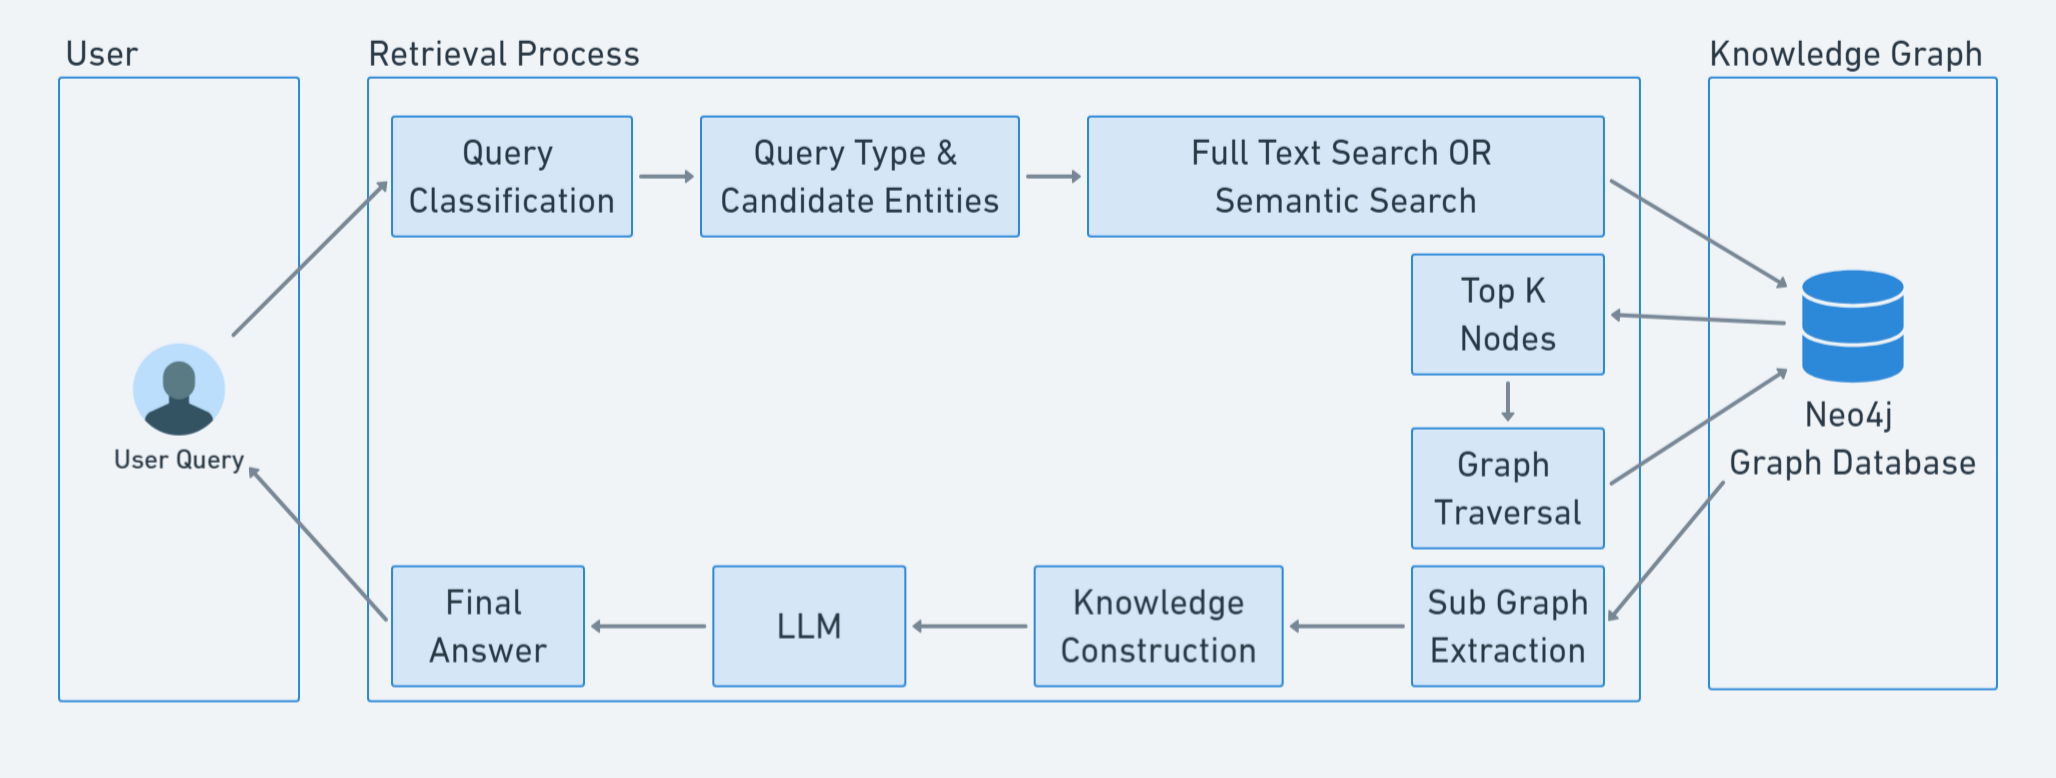
\includegraphics[width=0.45\textwidth]{knowledge-retrieval-pipeline.png}}
    \caption{Knowledge Retrieval and generation pipeline.}
    \label{fig:knowledge-retrieval-pipeline}
\end{figure}

\begin{itemize}
    \item Query Classification: The user's query is first analyzed by an LLM to classify its intent as either an entity\_query (seeking information about a single concept, e.g., "What is depression?") or a path\_query (exploring the relationship between multiple concepts, e.g., "How does CBT treat anxiety?").
          The LLM also extracts key entities from the query used for search keyword.

    \item Hybrid Search: The system identifies initial candidate nodes in the KG using a hybrid search strategy.
          It first attempts a fast full-text search for text matches.
          If unsuccessful, it falls back to a semantic vector search to find the most conceptually similar nodes.

    \item Adaptive Graph Traversal: Based on the query classification, an appropriate graph traversal algorithm is selected to gather relevant context:
          For entity\_query, a one-hop Neighbor Expansion is used to retrieve the central node and its immediate neighbors, effectively gathering its defining attributes and direct relationships.
          For path\_query, an N-Shortest Path algorithm is used to find the most direct connection(s) between the multiple entities identified in the query.

    \item Context Transformation \& Generation: The retrieved subgraph (nodes and edges) is transformed into a structured, human-readable text format. This context, along with the original query, is passed to the LLM, which generates the final, evidence-based answer for the user.
\end{itemize}

\section{Performance Evaluation}
\subsection{Experimental Setup}
To evaluate our system, we created a synthetic dataset of 433 question-answer pairs derived from our knowledge corpus (Knowledge Graph and original documents) using OpenAI o4-mini, ensuring the evaluation model was different from the one used in our pipeline to avoid bias.
We compared a Naive RAG system (using standard document chunks and vector search) as a baseline against four configurations of our KG-RAG system, which varied the search and traversal methods:

\begin{itemize}
    \item Default: Hybrid search with automatic traversal selection.

    \item Vector Search: Pure vector search for initial nodes.

    \item Neighbor Expansion: Forced neighbor expansion traversal.

    \item N-Shortest Path: Forced shortest path traversal.
\end{itemize}

\subsection{Retriever Performance}
We evaluated the quality of the context retrieved using Precision, Recall, Mean Reciprocal Rank (MRR), and Hit Ratio.
\begin{table}[htbp]
    \caption{Retriever evaluation}
    \begin{center}
        \begin{tabular}{|l|c|c|c|c|}
            \hline
            \textbf{Treatment}          & \textbf{Precision} & \textbf{Recall} & \textbf{MRR} & \textbf{Hit Ratio} \\
            \hline
            \textbf{Default}            & 0.1530             & 0.8203          & 0.3758       & 0.9053             \\
            \hline
            \textbf{Vector Search}      & 0.0603             & 0.5929          & 0.1737       & 0.6744             \\
            \hline
            \textbf{Neighbor Expansion} & 0.1123             & 0.8868          & 0.3191       & 0.9584             \\
            \hline
            \textbf{N-Shortest Path}    & 0.1245             & 0.5370          & 0.2788       & 0.6097             \\
            \hline
        \end{tabular}
        \label{tab:retrieval-evaluation-result}
    \end{center}
\end{table}

The results in Table~\ref{tab:retrieval-evaluation-result} show a clear trade-off.
The Default method achieved the highest precision and MRR, indicating it is best at returning highly relevant results at the top of the list.
However, Neighbor Expansion excelled in recall and hit ratio, demonstrating its superior ability to find all relevant information, even if it includes some noise.
Pure Vector Search performed poorly across all metrics.

\subsection{End-to-End System Performance}
We used the RAGAS framework to evaluate the quality of the final generated answers based on correctness, relevance, and faithfulness to the retrieved context \cite{es2024ragas}.

\begin{table}[htbp]
    \caption{Final answer evaluation}
    \begin{center}
        \begin{tabular}{|p{1.5cm}|c|c|c|c|}
            \hline
            \textbf{Treatment}          & \textbf{Similarity} & \textbf{Correctness} & \textbf{Relevancy} & \textbf{Faithfulness} \\
            \hline
            \textbf{Naive RAG}          & 0.9048              & 0.3391               & 0.6996             & 0.8993                \\
            \hline
            \textbf{Default}            & 0.9242              & 0.4155               & 0.8624             & 0.9435                \\
            \hline
            \textbf{Vector Search}      & 0.9115              & 0.3895               & 0.7387             & 0.8902                \\
            \hline
            \textbf{Neighbor Expansion} & 0.9248              & 0.4246               & 0.8723             & 0.9428                \\
            \hline
            \textbf{N-Shortest Path}    & 0.9033              & 0.3936               & 0.7900             & 0.4614                \\
            \hline
        \end{tabular}
        \label{tab:final-answer-evaluation-result}
    \end{center}
\end{table}

As shown in Table~\ref{tab:final-answer-evaluation-result},  the KG-RAG methods significantly outperformed the Naive RAG baseline.
The Neighbor Expansion strategy emerged as the overall best performer, demonstrating substantial improvements in key areas.
Specifically, it increased the Correctness score by 25.2\% (from 0.3391 to 0.4246) and the Relevancy score by 24.7\% (from 0.6996 to 0.8723) compared to the baseline.
Conversely, the extremely low Faithfulness score for N-Shortest Path (0.4614) highlights a critical finding: if the retrieval process fails to find a relevant path, the LLM is highly likely to hallucinate an answer, even if that answer seems plausible.
This underscores the vital importance of a robust and contextually appropriate retrieval mechanism for generating reliable responses.

\section{Conclusion}
This research successfully designed, implemented, and validated an optimized RAG architecture using a Knowledge Graph for a mental health chatbot.
Our findings demonstrate that this approach is superior to conventional RAG systems based on unstructured documents.
By leveraging a structured KG and an adaptive retrieval strategy, our system produces answers that are more accurate, relevant, and faithful to the source knowledge, thereby minimizing the risk of harmful misinformation.
The Neighbor Expansion traversal strategy proved to be the most effective method for retrieving comprehensive context that leads to high-quality final answers.
Future work could explore more advanced graph structures and evaluate the clinical impact of the chatbot with human users.

%Please number citations consecutively within brackets \cite{b1}. The 
%sentence punctuation follows the bracket \cite{b2}. Refer simply to the reference 
%number, as in \cite{b3}---do not use ``Ref. \cite{b3}'' or ``reference \cite{b3}'' except at 
%the beginning of a sentence: ``Reference \cite{b3} was the first $\ldots$''
%
%Number footnotes separately in superscripts. Place the actual footnote at 
%the bottom of the column in which it was cited. Do not put footnotes in the 
%abstract or reference list. Use letters for table footnotes.
%
%Unless there are six authors or more give all authors' names; do not use 
%``et al.''. Papers that have not been published, even if they have been 
%submitted for publication, should be cited as ``unpublished'' \cite{b4}. Papers 
%that have been accepted for publication should be cited as ``in press'' \cite{b5}. 
%Capitalize only the first word in a paper title, except for proper nouns and 
%element symbols.
%
%For papers published in translation journals, please give the English 
%citation first, followed by the original foreign-language citation \cite{b6}.



\bibliography{references}{}
\bibliographystyle{IEEEtran}

%\begin{thebibliography}{00}
%\bibitem{b1} G. Eason, B. Noble, and I. N. Sneddon, ``On certain integrals of Lipschitz-Hankel type involving products of Bessel functions,'' Phil. Trans. Roy. Soc. London, vol. A247, pp. 529--551, April 1955.
%\bibitem{b2} J. Clerk Maxwell, A Treatise on Electricity and Magnetism, 3rd ed., vol. 2. Oxford: Clarendon, 1892, pp.68--73.
%\bibitem{b3} I. S. Jacobs and C. P. Bean, ``Fine particles, thin films and exchange anisotropy,'' in Magnetism, vol. III, G. T. Rado and H. Suhl, Eds. New York: Academic, 1963, pp. 271--350.
%\bibitem{b4} K. Elissa, ``Title of paper if known,'' unpublished.
%\bibitem{b5} R. Nicole, ``Title of paper with only first word capitalized,'' J. Name Stand. Abbrev., in press.
%\bibitem{b6} Y. Yorozu, M. Hirano, K. Oka, and Y. Tagawa, ``Electron spectroscopy studies on magneto-optical media and plastic substrate interface,'' IEEE Transl. J. Magn. Japan, vol. 2, pp. 740--741, August 1987 [Digests 9th Annual Conf. Magnetics Japan, p. 301, 1982].
%\bibitem{b7} M. Young, The Technical Writer's Handbook. Mill Valley, CA: University Science, 1989.
%\end{thebibliography}



\end{document}
